
%(BEGIN_QUESTION)
% Copyright 2011, Tony R. Kuphaldt, released under the Creative Commons Attribution License (v 1.0)
% This means you may do almost anything with this work of mine, so long as you give me proper credit

The following temperature control system is all-pneumatic, with a pneumatic transmitter, controller, and air-to-close control valve.  Your task is to sketch the necessary tube and wire connections so that the control valve will go to its ``fail-safe'' position when an operator presses the pushbutton:

$$\includegraphics[width=15.5cm]{i01447x01.eps}$$

The system is currently drawn without the shutdown solenoid connected at all.  Feel free to ``break'' and re-route any existing tubes as necessary to modify this system so that it includes the solenoid valve, and will bypass the controller's output signal when the button is pressed.
 
\underbar{file i01447}
%(END_QUESTION)





%(BEGIN_ANSWER)

Everything must be correct in the diagram to receive credit: the switch using its NC contact (de-energizing when pushed), with the valve tube connected to ``C'', the controller to ``P'', and ``E'' vented:

$$\includegraphics[width=15.5cm]{i01447x02.eps}$$

An alternative where the solenoid valve stops and vents air from the controller's supply tube is equally workable, and worth full credit.

An alternative method where ``P'' is vented and ``E'' goes to the controller would also work if the switch is wired NO.  However, this solution should be granted only 8 points, not the full 10 (since this is not the standard usage of P, C, and E ports on a three-way valve).

If a student suggests a solution that would vent air from the valve, but only by directly venting supply pressure to atmosphere, grant only half-credit (5 points).  Such a solution would indeed cause the valve to go to its fail position, but it would be very impractical and wasteful of instrument air. 

%(END_ANSWER)





%(BEGIN_NOTES)

{\bf This question is intended for exams only and not worksheets!}.

%(END_NOTES)


